

\section{Introduction} 

Compared with supervised learning, 
the shared difficulty of various forms of unsupervised learning is the lack of 
\emph{paired} input/output data  
with which standard regression or classification tasks can be invoked. 
The gist of 
most unsupervised methods is to 
find, in one way or another,  meaningful correspondences between 
points from two distributions. 
For example, generative models such as 
generative adversarial networks (GAN) 
and variational autoencoders (VAE) 
\cite[e.g.,][]{goodfellow2014generative, kingma2013auto, dinh2016density}
seek to 
map data points 
to latent codes 
following 
a simple elementary (Gaussian) distribution
with which the data can be generated and manipulated. 
Representation learning 
rests on the idea that 
if a sufficiently smooth function can map
a structured data distribution to an elementary 
distribution, it can (likely) be endowed 
with certain  semantically meaningful interpretation
and useful for various downstream learning tasks.  
On the other hand, 
domain transfer methods 
find mappings to transfer points 
from two different data distributions, 
both observed empirically, 
for the purpose of image-to-image translation,  %
style transfer, and domain adaption \citep[e.g.,][]{cyclegan, flamary2016optimal, trigila2016data, peyre2019computational}.
All these tasks can be framed  unifiedly %
as finding a transport map between two distributions: 

\noindent\textbf{The Transport Mapping Problem}  
\emph{Given empirical observations 
of two distributions $X_0\sim \tg_0,  X_1\sim \tg_1$ on $\RR^d$, 
find a %
transport map $T\colon\RR^d\to\RR^d$ (hopefully nice or optimal in certain sense),  
such that $Z_1 \defeq T(Z_0)\sim \tg_1$ when $Z_0 \sim \tg_0$, that is, $(Z_0,Z_1)$ is a coupling (a.k.a transport plan) of $\tg_0$ and $\tg_1$.  
}



Several lines of techniques have been developed depending on how to  represent and train  the map $T$. 
In traditional generative models, 
$T$ 
is parameterized as a neural network, 
and trained with either 
GAN-type minimax algorithms or (approximate) maximum likelihood estimation (MLE).  
However, GANs are known to suffer from numerically instability  and mode collapse issues,  
and require substantial engineering efforts 
and human tuning, which often do not transfer well across different model architecture and datasets.  
On the other hand, MLE tends to be intractable for complex models, 
and hence
requires 
approximate variational or Monte Carlo inference techniques  
such as those used in variational auto-encoders (VAE), 
or special model structures  
such as normalizing flow and auto-regressive models, to yield tractable likelihood, causing  difficult trade-offs between expressive power and computational cost. %



Recently, advances have been made by representing 
the transport plan 
\emph{implicitly as a continuous time  process}, such as 
flow models with neural ordinary differential equations (ODEs) \citep[e.g.,][]{chen2018neural, papamakarios2021normalizing} and  diffusion models by stochastic differential equations (SDEs) \citep[e.g.,][]{song2020score, ho2020denoising, tzen2019theoretical, de2021diffusion, vargas2021solving};
in these models, 
a neural network 
is trained to represent the 
drift force of the processes
and a numerical ODE/SDE solver is used to simulate the process during inference. 
The key idea is that, 
by leveraging the mathematical structures of ODEs/SDEs, 
the continuous-time models 
can be trained efficiently without 
resorting to minimax or traditional approximate inference techniques. 
The most notable examples are 
the recent score-based generative models \cite{song2019generative, song2020improved, song2020score} 
and denoising diffusion probabilistic models (DDPM) \citep{ho2020denoising}, 
which we call denoising diffusion methods collectively. 
These methods 
allow us to train 
large-scale diffusion/SDE-based generative models that 
surpass GANs on image generation in both image quality and diversity,
without the instability and mode collapse issues
\citep[e.g.,][]{dhariwal2021diffusion, glide, dalle2, imagegen}.  
The learned SDEs can be converted into deterministic ODE models  for faster inference with the method of probability flow ODEs \citep{song2020score} and DDIM \citep{song2020denoising}. 

However, compared with the traditional one-step models like GAN and VAE, 
a key drawback of  continuous-times models %
is the 
high computational cost in inference time: drawing a single point (e.g., image) requires to solve the ODE/SDE with a numerical solver that needs to repeatedly call the expensive neural drift function. 
In addition, the existing denoising diffusion techniques 
require substantial hyper-parameter search in an involved design space 
and are still poorly understood both empirically and theoretically \citep{elucidating}. 



In existing approaches, generative modeling and domain transfer 
are  typically treated  separately. 
It often requires to extend or customize a generative learning techniques to solve domain transfer problems; see e.g., Cycle GAN \citep{cyclegan} and diffusion-based image-to-image translation \citep[e.g.,][]{su2022dual, zhao2022egsde}. 
One framework that naturally unifies both domains is 
 optimal transport (OT)  \citep[e.g.,][]{villani2021topics,ambrosio2021lectures,figalli2021invitation,peyre2019computational}, which 
endows a collection of techniques for finding optimal
couplings with minimum transport costs of form 
$\E[c(Z_1-Z_0)]$ w.r.t. a cost function $c\colon \RR^d\to \RR$, yielding 
natural applications  to both generative and transfer learning. 
However, 
the existing OT techniques 
are slow for problems with high dimensional and large volumes of data \citep{peyre2019computational}. 
Furthermore, 
as the transport costs do not perfectly align with 
the actual learning performance, 
methods that faithfully find the optimal transport maps 
do not necessarily have better learning performance \citep{korotin2021neural}. 





\begin{figure}[h]
    \centering
    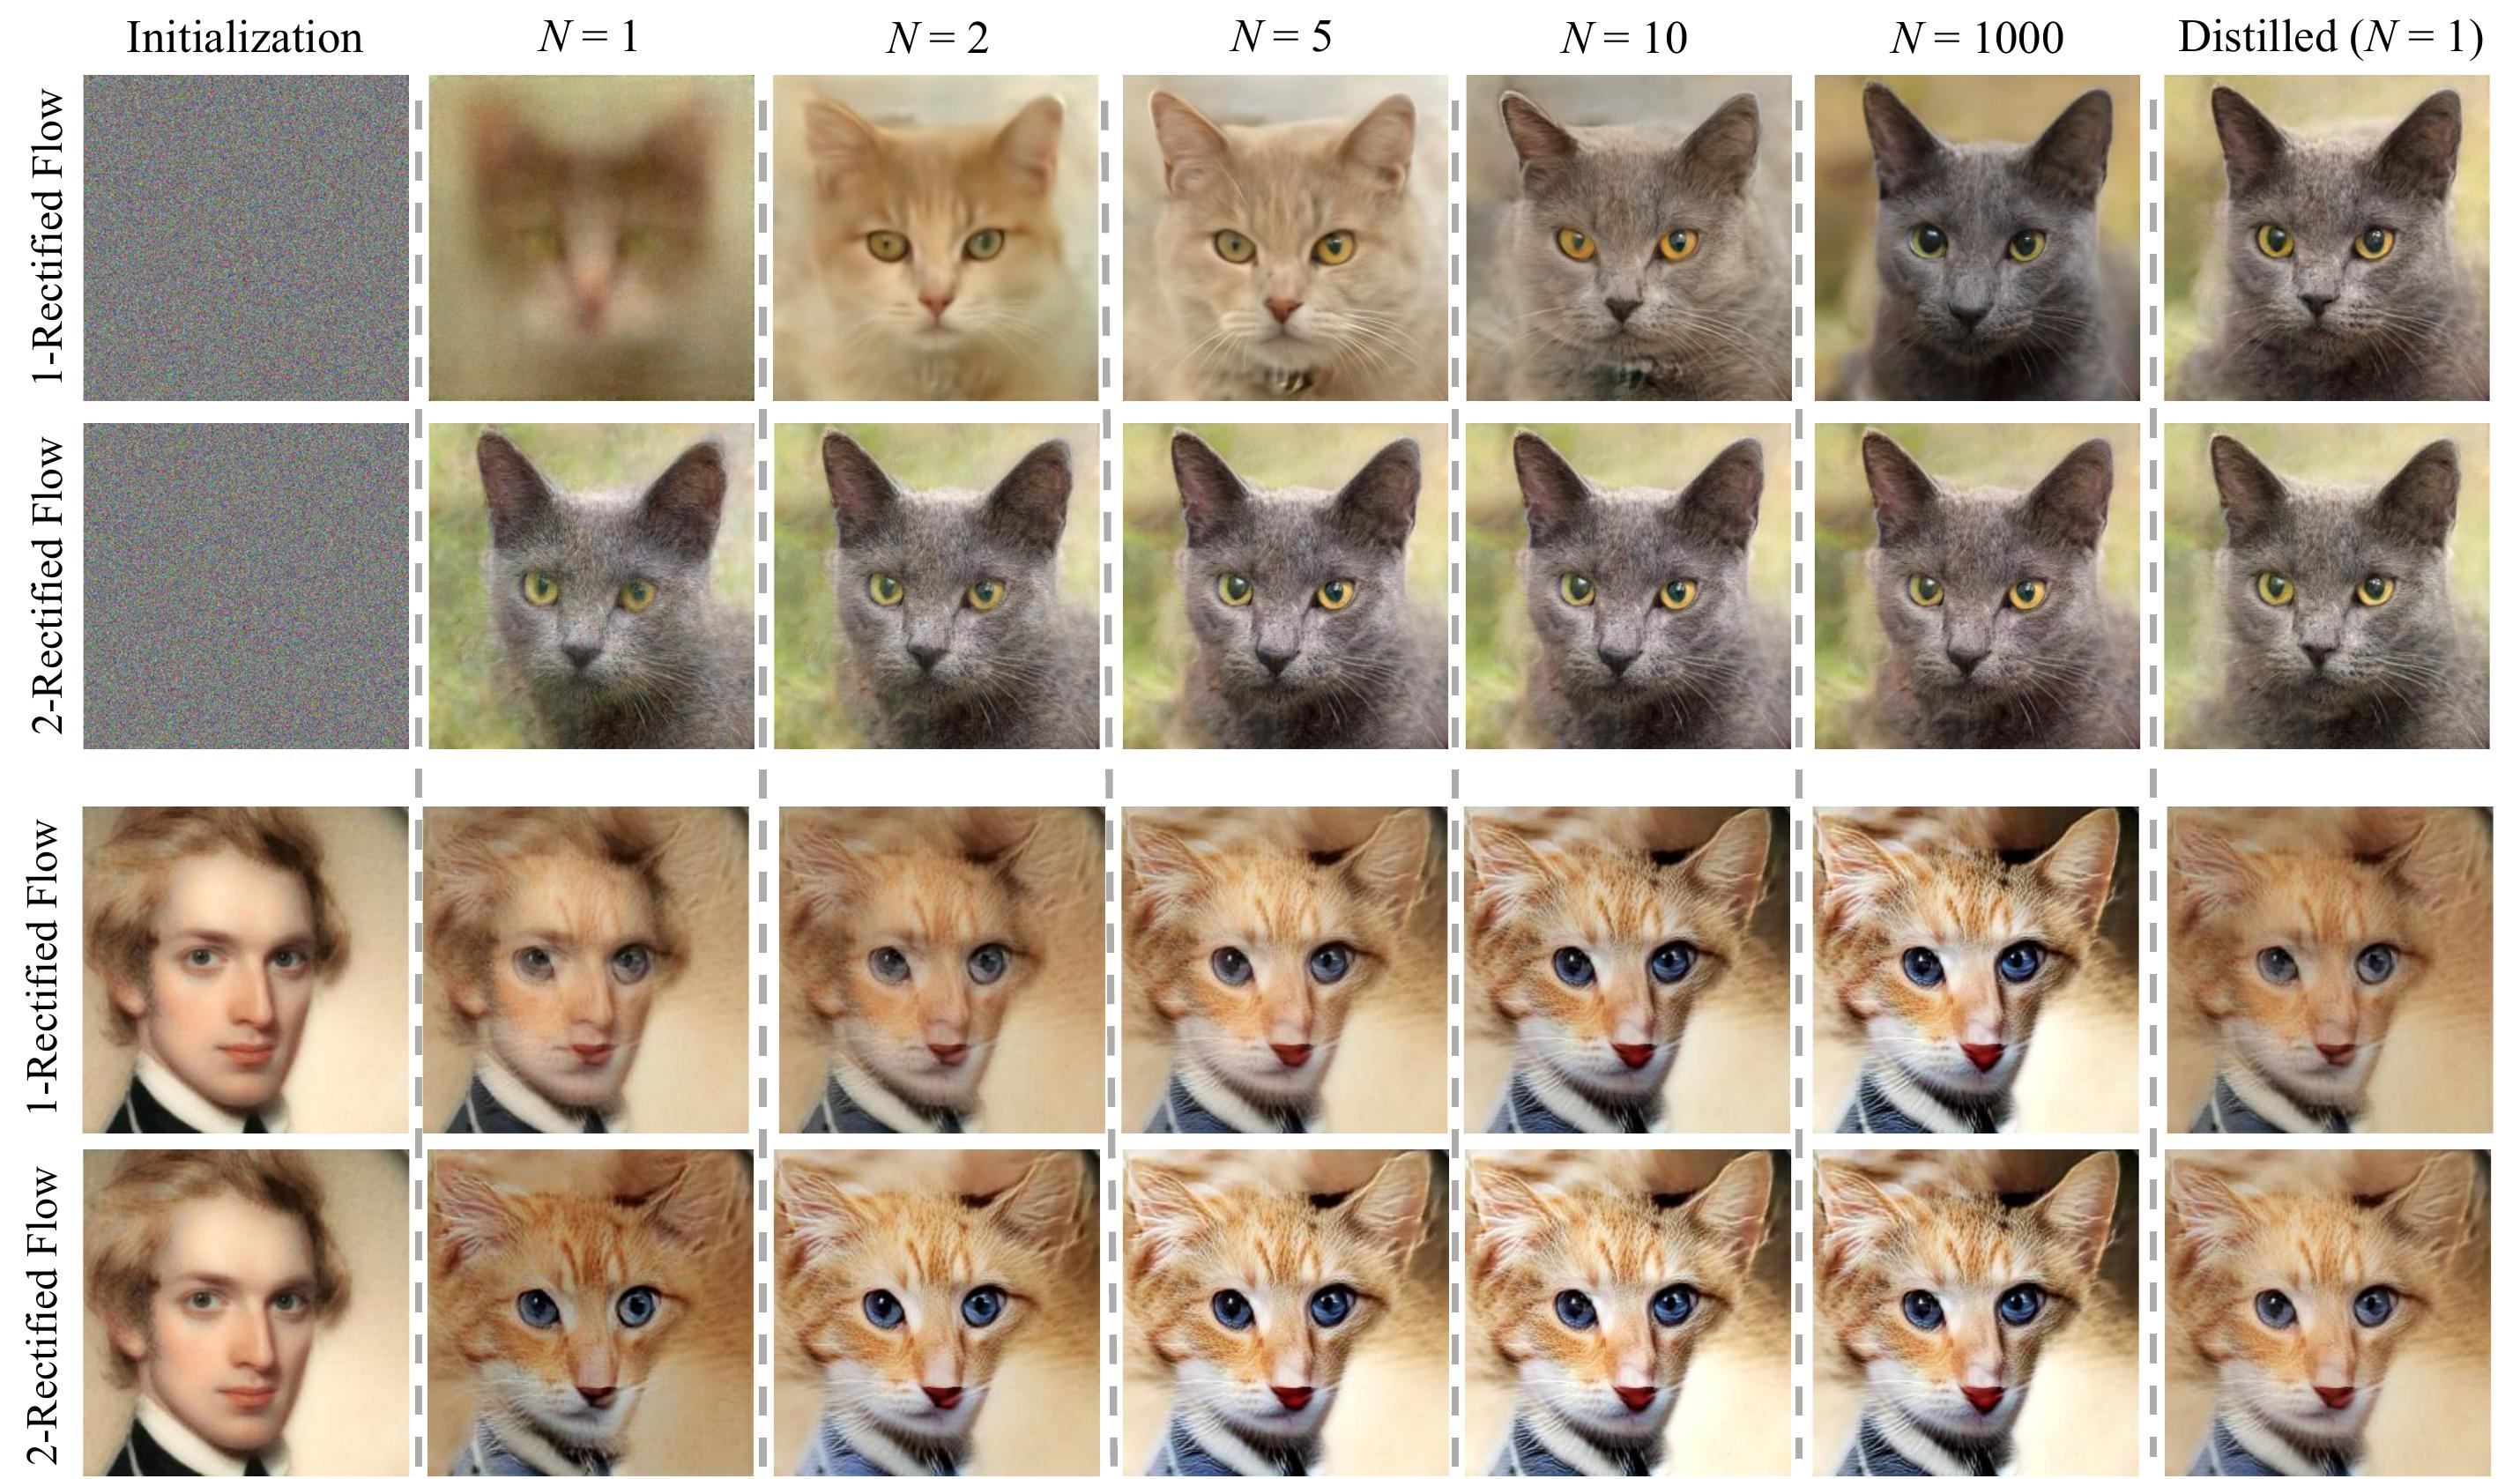
\includegraphics[width=0.95\textwidth]{arxiv_figures/cat_triangle_new_2_cy.pptx.jpeg} %
    \caption{The trajectories of rectified flows for 
    image generation 
    ($\tg_0$: standard Gaussian noise,  $\tg_1$: cat faces, top two rows), 
    and image transfer between human and cat faces ($\tg_0$: human faces,  $\tg_1$: cat faces, bottom two rows), 
    when simulated using Euler method with step size $1/N$ for $N$ steps. 
    The first rectified flow induced from the training data (\emph{1-rectified flow}) yields good results with a very small number (e.g., $\geq 2$) of steps; 
   the straightened reflow induced from \emph{1-rectified flow} (denoted as \emph{2-rectified flow})   
   has nearly straight line trajectories and yield good results even with one  discretization step. 
    }
    \label{fig:cat_k}
\end{figure}


\subsection*{Contribution}
We introduce 
\emph{rectified flow}, 
a surprisingly  
simple approach  
to the transport mapping problem, 
which unifiedly solves both 
generative modeling and domain transfer. 
The rectified flow 
is an ODE model 
that transport 
distribution $\tg_0$ to $\tg_1$
by 
\emph{following straight line paths as much as possible.} 
The straight paths 
are preferred both theoretically 
because it is the shortest path 
between two end points, 
and computationally because it can be 
exactly simulated without time discretization. 
Hence,
 flows  with straight paths 
bridge the gap between one-step and continuous-time models. %

Algorithmically, the rectified flow 
is trained with 
a simple and scalable unconstrained 
least squares optimization procedure,    which 
avoids the instability issues of GANs,  
the intractable likelihood of MLE methods, and the subtle hyper-parameter decisions of denoising diffusion models.  
The procedure of obtaining the rectified flow from the training data has the attractive theoretical property of 
1) yielding a coupling with 
non-increasing transport cost jointly for all convex cost $c$, 
and 2) making the paths of flow increasingly straight and hence incurring lower error with numerical solvers.
Therefore, 
with a \emph{reflow} 
procedure that iteratively trains new 
rectified flows
with the data simulated from the previously obtained rectified flow, 
we obtain nearly straight flows 
that yield good results even with
the coarsest time discretization, i.e., 
one Euler step. 
Our method is purely ODE-based, 
and is both conceptually simpler and practically faster in inference time than the SDE-based approaches of
\cite{ho2020denoising, song2020score, song2020denoising}. 

Empirically, 
rectified flow 
can yield
high-quality results 
for image generation when simulated with a very few number of Euler steps (see Figure~\ref{fig:cat_k}, top row).
Moreover, with just one step of reflow, 
the flow becomes nearly straight and hence yield good results with a single Euler discretization step (Figure~\ref{fig:cat_k}, the second row).
This substantially improves 
over the standard denoising diffusion methods. %
Quantitatively, we claim a state-of-the-art result of FID (4.85) and recall (0.51) on CIFAR10 for one-step fast diffusion/flow models~\citep{bao2022analytic, lyu2022accelerating, xiao2021tackling, zheng2022truncated, luhman2021knowledge}. 
The same algorithm 
also achieves superb result on domain transfer tasks such as image-to-image translation (see the bottom two rows of Figure \ref{fig:cat_k}) and 
transfer learning. 






  


\section{Method} 
We provide a quick overview of the method in Section~\ref{sec:firstintro}, 
followed with some discussion and remarks in Section~\ref{sec:secondintro}. 
We introduce a nonlinear extension of our method in Section~\ref{sec:nonlinear}, 
with which we clarify the connection and advantages of our method with the method of probability flow ODEs \citep{song2020score} and DDIM \citep{song2020denoising}. 


\begin{figure}[t]
\hspace{-1em}
\begin{tabular}{wl{0.17\textwidth}wl{0.3\textwidth}wl{0.17\textwidth}wl{0.17\textwidth}wl{0.15\textwidth}wl{0.1\textwidth}} 
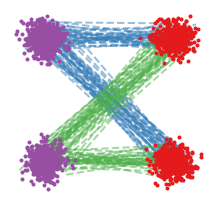
\includegraphics[width=.15\textwidth]{arxiv_figures/cross22_dash.png}  &
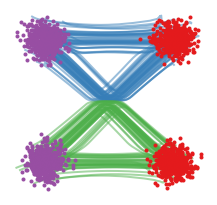
\includegraphics[width=.15\textwidth]{arxiv_figures/cross12.png} 
\raisebox{1em}{{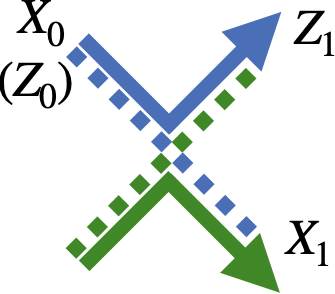
\includegraphics[width=.12\textwidth]{arxiv_figures/arrowsdfd.png}}}%
\hspace{-2em} 
 & 
 \hspace{-2em} 
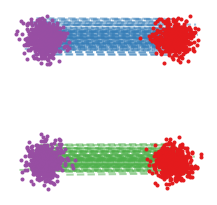
\includegraphics[width=.15\textwidth]{arxiv_figures/cross32_dash.png} 
 & 
 \hspace{-2em} 
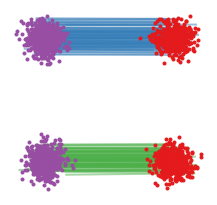
\includegraphics[width=.15\textwidth]{arxiv_figures/cross42.png} 
 & 
 \hspace{-3.5em}
\raisebox{1.2em}{\fbox{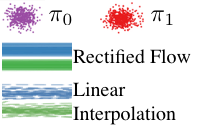
\includegraphics[width=.15\textwidth]{arxiv_figures/cross_legend.png}}} 
 & 
\\
\begin{tabular}{l} 
\scriptsize (a) Linear interpolation \\ 
\scriptsize $X_t = tX_1+(1-t)X_0$  
\end{tabular} 
& 
\begin{tabular}{l} 
\scriptsize (b)  Rectified flow $Z_t$ \\ 
\scriptsize induced by $(X_0,X_1)$ 
\end{tabular} 
 & 
  \hspace{-2em} 
\begin{tabular}{l} 
\scriptsize (c) Linear interpolation \\ 
\scriptsize $Z_t = tZ_1+(1-t)Z_0$   
\end{tabular} 
& 
  \hspace{-2em} 
\begin{tabular}{l} 
\scriptsize (d)  Rectified flow $Z'_t$ \\ 
\scriptsize induced by $(Z_0,Z_1)$ 
\end{tabular} 
&  
& 
\end{tabular}
\caption{(a) Linear interpolation of data input $(X_0,X_1)\sim \tg_0\times \tg_1$. 
(b) The rectified flow $Z_t$ induced by $(X_0,X_1)$;  
the trajectories are ``rewired" at the intersection points 
to avoid the crossing. 
 (c) The linear interpolation of the end points $(Z_0,Z_1)$ of flow $Z_t$.
 (d) The rectified flow induced from $(Z_0,Z_1)$, which  follows straight paths. 
}
\label{fig:twodotstoy}
\end{figure}

\subsection{Overview}%
\label{sec:firstintro}

\paragraph{Rectified flow}
Given empirical observations of $X_0\sim \tg_0, X_1\sim \tg_1$, 
the rectified flow induced from $(X_0,X_1)$ 
is an ordinary differentiable model (ODE)
on time $t\in[0,1]$, 
$$
\d Z_t = v(Z_t, t) \dt, 
$$
which converts $Z_0$ from $\tg_0$ to a $Z_1$ following $\tg_1$. 
The drift force 
 $v\colon \RR^d\to \RR^d$  is set to drive the flow to 
 follow the direction $(X_1-X_0)$ 
 of the linear path pointing from $X_0$ to $X_1$
 as much as possible, by solving a simple 
 least squares regression problem:  \bbb\label{equ:mainf}
\min_{v} %
\int_0^1\E \left [ \norm{( X_1 - X_0) - v\big (X_t,~ t\big)}^2
\right ] \dt, 
~~~~~\text{with}~~~~
X_t = t X_1 + (1-t) X_0, 
\eee 
where $X_t$ is 
the linear interpolation  of  $X_0$ and  $X_1$. 
Naviely, $X_t$ follows the ODE of $\d  X_t =(X_1-X_0)\dt,$ which is non-causal (or anticipating) as the update of $X_t$ requires the information of the final point $X_1$.  
By fitting the drift $v$ with $X_1-X_0$, 
the rectified flow \emph{causalizes}
the paths of linear interpolation $X_t$, 
yielding an ODE flow %
that can be simulated without seeing the future. %


 In practice, we parameterize $v$ with a neural network or other nonlinear models 
 and solve  
  \eqref{equ:mainf} %
  with any  off-the-shelf stochastic optimizer, such as stochastic gradient descent,  
  with empirical draws of $(X_0,X_1)$. See 
  Algorithm~\ref{alg:cap}. 
  After we get $v$, we solve the ODE starting from $Z_0 \sim \tg_0$ to transfer $\tg_0$ to $\tg_1$,
   backwardly starting from $Z_1\sim \tg_1$ to transfer $\tg_1$ to $\tg_0$. Specifically, 
  for  backward sampling, 
  we simply  
  solve $\d \tilde X_t = -v(\tilde X_t, t) \dt $ initialized from $\tilde X_0 \sim \tg_1$ and set 
   $X_t= \tilde X_{1-t}$. 
   The forward and backward sampling 
are equally favored by the training  algorithm, because  the objective  in \eqref{equ:mainf} is 
\emph{time-symmetric} 
in that it yields the equivalent problem if we exchange $X_0$ and $X_1$ and flip the sign of $v$. 



 





\paragraph{Flows avoid crossing} %
A key to understanding the method is the non-crossing property of flows: 
the different paths 
following a well defined ODE $\d Z_t = v(Z_t,t) \dt $, 
whose solution exists and is unique, \emph{cannot cross each other} at any time $t\in[0,1)$. 
Specifically,
there exists no location $z\in\RR^d$ and time $t\in[0,1)$, such that two paths go across $z$ at time $t$ along different directions, because otherwise the solution of the ODE would be non-unique. 
On the other hand, the paths of the interpolation process $X_t$ may intersect with each other (Figure~\ref{fig:twodotstoy}a), which makes it non-causal. 
Hence, %
as shown in Figure~\ref{fig:twodotstoy}b,  
the rectified flow 
\emph{rewires} the individual trajectories passing through the intersection points to avoid crossing, while
tracing out the same density map as the linear interpolation paths
due to the optimization of 
\eqref{equ:mainf}.  
We can view the linear interpolation $X_t$ as building
 roads (or tunnels) to connect $\tg_0$ and $\tg_1$, 
 and the rectified flow as traffics of particles passing through the roads in a myopic, memoryless, non-crossing way, 
 which allows them to ignore the global  
 path information of how $X_0$ and $X_1$ are paired, 
 and rebuild a more deterministic pairing of $(Z_0,Z_1)$. 


\paragraph{Rectified flows reduce transport costs} 
If \eqref{equ:mainf} is solved exactly, 
the pair $(Z_0,Z_1)$ 
of the rectified flow 
is guaranteed to be a valid coupling of $\tg_0,\tg_1$ (Theorem~\ref{thm:marginal}), 
that is, $Z_1$ follows $\tg_1$ if $Z_0\sim \tg_0$.  
Moreover, $(Z_0,Z_1)$ guarantees to yield no larger transport cost than the data pair $(X_0,X_1)$ simultaneously for \emph{all} convex cost functions $c$ (Theorem~\ref{thm:cost}). 
The data pair $(X_0,X_1)$ can be an arbitrary coupling of $\tg_0,\tg_1$, typically independent  (i.e., $(X_0,X_1)\sim \tg_0\times \tg_1$)  
as dictated by the lack of meaningfully paired observations in practical problems. %
In comparison, 
the rectified coupling $(Z_0,Z_1)$ has a deterministic dependency as it is constructed from an ODE model. 
Denote by $(Z_0,Z_1)=\rectify((X_0,X_1))$ 
the mapping from $(X_0,X_1)$ to $(Z_0,Z_1)$. 
Hence, %
$\rectify(\cdot)$ converts an arbitrary coupling into a deterministic coupling with lower convex transport costs. 








 



\paragraph{Straight line flows yield fast simulation}
Following Algorithm~\ref{alg:cap}, 
denote by $\vv Z = \rectifyflow((X_0,X_1))$ the rectified flow induced from $(X_0,X_1)$. 
Applying this operator recursively 
yields a sequence of rectified  flows 
$\vv Z^{k+1} = \rectifyflow((Z_0^k, Z_1^k))$ with $(Z_0^0,Z_1^0)=(X_0,X_1)$, where $\vv Z^k$ is the $k$-th rectified flow, or simply \emph{$k$-rectified flow}, induced from $(X_0,X_1)$. 

This 
\emph{reflow} 
procedure %
not only decreases transport cost,
but also has the important effect of 
straightening paths of rectified flows, 
that is, making the paths of the flow more straight. 
This is highly attractive computationally  
as flows with nearly straight paths 
incur small time-discretization error 
in numerical simulation. Indeed, perfectly straight paths can be simulated exactly with a single Euler step and is effectively a one-step model. 
This addresses the very bottleneck of high inference cost 
in existing continuous-time ODE/SDE models.  














\begin{algorithm}[t]
\caption{{\Name} Flow: Main Algorithm}\label{alg:cap}
\begin{algorithmic}
\STATE \textbf{Procedure}: $\vv Z={\rectifyflow((X_0,X_1))}$: 
\vspace{.2\baselineskip}


\STATE~~~\emph{Inputs}: Draws from a coupling $(X_0,X_1)$ of $\tg_0$ and $\tg_1$; velocity model $v_\theta \colon \RR^d \to \RR^d$ with parameter $\theta.$ 
\vspace{.155\baselineskip}
\STATE~~\emph{Training}:
$
\displaystyle 
\hat \theta = \argmin_\theta
\E\left [\norm{X_1 - X_0 - v(t X_1 +(1-t)X_0, ~t )}^2 \right], 
$
with $t \sim \uniform([0,1])$.
\vspace{.15\baselineskip}


\STATE~~\emph{Sampling}: Draw $(Z_0,Z_1)$ following $\d Z_t = v_{\hat\theta}(Z_t,t)\dt$ starting from $Z_0 \sim \tg_0$ (or backwardly $Z_1\sim \tg_1$).


\STATE~~\emph{Return}: $\vv Z = \{Z_t\colon t\in[0,1]\}$.
\vspace{.4\baselineskip}


\STATE \textbf{Reflow} (optional): $%
\vv Z^{k+1} = \rectifyflow((Z_0^k, Z_1^k))$, starting from $(Z^0_0,Z^0_1) = (X_0,X_1)$.
\vspace{.2\baselineskip}

\STATE \textbf{Distill} (optional): Learn a neural network $\hat T$ to distill the $k$-rectified flow, such that $Z^k_1 \approx \hat T(Z^k_0)$. 
\end{algorithmic}
\end{algorithm}



 


 
 





 
 
 \subsection{Main Results and Properties} 
 \label{sec:secondintro}

We provide more in-depth discussions 
on the main properties of  rectified flow. 
We keep the discussion informal 
to highlight the intuitions  in this section and defer the 
  full course theoretical analysis to  Section~\ref{sec:theory}. %
 
 First, 
 for a given input coupling $(X_0,X_1)$, 
it is easy to see that the exact minimum of \eqref{equ:mainf} is achieved if 
 \bbb \label{equ:vxoracle}
 v^X(x,t) = \E[X_1- X_0 ~|~ X_t=x],
 \eee 
 which is the expectation of the line directions $X_1-X_0$ that pass through $x$ at time $t$. 
 We discuss below the property of rectified flow $\d Z_t = v^X(Z_t,t)\dt $ with $Z_0\sim \tg_0$,
 assuming that the ODE has an unique solution. %
 
 \paragraph{Marginal preserving property} [Theorem~\ref{thm:marginal}] \emph{The pair $(Z_0,Z_1)$ is a coupling of $\tg_0$ and $\tg_1$. 
In fact, the marginal law of $Z_t$ equals that of $X_t$ at every time  $t$, that is, $\law(Z_t)=\law(X_t), \forall t\in[0,1]$. } 

Intuitively, this is because, by the definition of $v^X$ in \eqref{equ:vxoracle}, the expected amount of mass
that  passes through every infinitesmal volume at all location and time are equal under the dynamics of $X_t$ and $Z_t$, which ensures that they trace out the same marginal distributions: \newcommand{\imineq}[2]{\vcenter{\hbox{\includegraphics[height=#2ex]{#1}}}}
\bb 
\text{
Flow in $\&$ out}\!\left(\imineq{arxiv_figures/arrow11_new.png}{6} \right) \!\! = 
\text{Flow in $\&$ out}\!\left(\imineq{arxiv_figures/arrow22_new.png}{6} \right)\!, ~\forall \text{time $\&$ location} 
&&\implies && \law(Z_t)=\law(X_t),\forall t.%
\ee 
On the other hand, the joint distributions of the whole trajectory of $Z_t$ and that of $X_t$ are  different in general.  
In particular, $X_t$ is in general a non-causal, non-Markov process, 
with $(X_0,X_1)$ a stochastic coupling,
and $Z_t$  \emph{causalizes}, \emph{Markovianizes}
 and \emph{derandomizes} $X_t$, while preserving the marginal distributions at all time.  



\paragraph{Reducing  transport costs} [Theorem~\ref{thm:cost}] \emph{The coupling $(Z_0,Z_1)$ yields lower or equal convex transport costs than the input $(X_0,X_1)$ in that  $\E[c(Z_1-Z_0)] \leq \E [c(X_1 - X_0)]$ for any convex cost $c\colon \RR^d\to \RR$. }

 
The transport costs measure the expense of transporting the mass of one distribution to another following the assignment relation specified by the coupling and is a central topic in optimal transport \citep[e.g.,][]{villani2009optimal,villani2021topics, santambrogio2015optimal, peyre2019computational, figalli2021invitation}. %
Typical examples are $c(\cdot)= \norm{\cdot}^\alpha$ with $\alpha\geq 1$.
Hence, $\rectify(\cdot)$
yields a Pareto descent on the collection of all convex transport costs, without targeting any specific $c$. 
This distinguishes it from the 
typical optimal transport optimization methods, which are explicitly framed 
to optimize a given $c$. 
As a result, recursive application of $\rectify(\cdot)$  
does not guarantee to attain the $c$-optimal coupling for any given $c$, with the exception 
in the one-dimensional case when the fixed point of $\rectify(\cdot)$ coincides with the unique monotonic coupling that simultaneously minimizes all non-negative convex costs $c$; see Section~\ref{sec:stcouplings}. 

Intuitively, 
the convex transport costs 
are guaranteed to decrease because the paths of the rectified flow $Z_t$ is a rewiring of the straight paths connecting $(X_0,X_1)$. 
To give an illustration, %
consider the simple case of $c(\cdot) = \norm{\cdot}$ when transport costs $\E[\norm{X_0-X_1}]$ and $\E[\norm{Z_0-Z_1}]$  
 are the expected length of the straight lines connecting the end points. 
 The inequality can be proved graphically as follows: 
$$
\text{ 
$\E[\norm{Z_0-Z_1}]$
$= $ 
Length$\left(\imineq{arxiv_figures/=.png}{6}\right)$ 
$\overset{\scriptsize (*)}{\leq}$
Length$\left(\imineq{arxiv_figures/v2.png}{6}\right)$ %
$\overset{\scriptsize (**)}{=}$ Length$\left(\imineq{arxiv_figures/x.png}{6}\right)$
$=$ %
${\E[\norm{X_0-X_1}]}$
}, 
$$
where $\overset{\scriptsize (*)}{\leq}$ uses 
the triangle inequality,
and $\overset{\scriptsize(**)}{=}$ holds because the paths of $Z_t$ is a rewiring 
of the straight paths of $X_t$, following the 
construction of $v^\X$ in \eqref{equ:vxoracle}.  
For general convex $c$, 
a similar proof using Jensen's inequality is shown in Section~\ref{sec:cost}. 





\paragraph{Reflow, straightening, fast simulation} 
As shown in Figure~\ref{fig:toystar}, 
when we recursively apply the procedure $\vv Z^{k+1} = \rectifyflow((Z_0^k, Z_1^k))$, 
 the paths of the $k$-rectified flow $\vv Z^k$ 
are increasingly 
straight, and hence easier to simulate numerically, as $k$ increases.  %
This straightening tendency can be guaranteed theoretically. 

\begin{figure}[h]
~~~~~~
\begin{tabular}{wc{0.15\textwidth}wc{0.32\textwidth}wc{0.22\textwidth}wc{0.2\textwidth}}
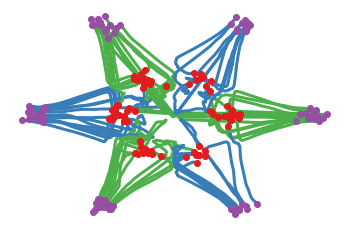
\includegraphics[height=.18\textwidth]{arxiv_figures/circle06h0p1_v2_0.png} \hspace{-.05\textwidth} & 
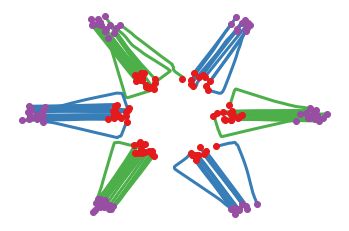
\includegraphics[height=.18\textwidth]{arxiv_figures/circle06h0p1_v2_1.png} & \hspace{-.05\textwidth} 
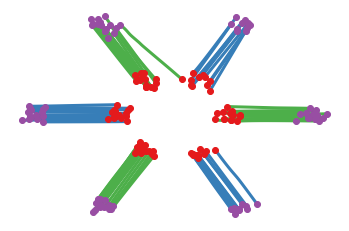
\includegraphics[height=.18\textwidth]{arxiv_figures/circle06h0p1_v2_2.png} & \hspace{-.00\textwidth} 
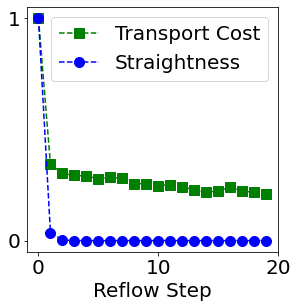
\includegraphics[height=.18\textwidth]{arxiv_figures/circle06h0p1_v2_loss.png}  \\
\begin{tabular}{l}
\small (a)The 1st rectified flow $\vv Z^1$ \\ %
\scriptsize $\vv Z^1=\rectifyflow((X_0,X_1))$
\end{tabular}
& 
\begin{tabular}{l}
\small (b) Reflow $\vv Z^2$ \\ %
\scriptsize $\vv Z^2=\rectifyflow((Z_0^1,Z_1^1))$
\end{tabular}
& 
\begin{tabular}{l}
\small (c)  Reflow $\vv Z^3$ \\ %
\scriptsize $\vv Z^3=\rectifyflow((Z_0^2,Z_1^2))$
\end{tabular}
&  
\begin{tabular}{l}
\small(d)
Transport cost, \\ %
\small Straightness
\end{tabular}
\end{tabular}
\definecolor{dotscolor1}{HTML}{984EA3}
\definecolor{dotscolor2}{HTML}{E41A1C}
\caption{(a)-(c) Samples of trajectories  drawn from the reflows on a toy example (\textcolor{black}{$\tg_0$: purple dots},
\textcolor{black}{$\tg_1$: red dots}; 
the green and blue lines are trajectories connecting different modes of $\tg_0,\tg_1$). 
(d) The
straightness and the relative L2 transport cost   v.s. 
the reflow steps; the values are scaled into $[0,1]$, so 0 corresponds to  straight lines and $L_2$ optimal transport; see Section~\ref{sec:toy} for more information.  %
We use the non-parametric model in \eqref{equ:npfunc} with bandwidth $h=0.1$. 
}
\label{fig:toystar}
\end{figure}

Specifically, 
we say that a flow $\d Z_t = v(Z_t, t)\dt$ %
is straight if we have almost surely that $Z_t = t Z_1 + (1-t) Z_0$ for $\forall t\in[0,1]$, 
or equivalently $v(Z_t,t)=Z_1-Z_0=\const$ following each path. 
(More precisely, ``straight'' here refers to  straight with a constant speed.) 
Such straight flows are highly attractive computationally 
as it is effective a one-step model: 
 a single Euler step update $Z_1 = Z_0 + v(Z_0,0)$ calculates the exact $Z_1$ from $Z_0$. %
 Note that the linear interpolation $\vv X= \{X_t\}$ is straight by this definition but it is not a (causal) flow and hence can not be simulated without an oracle assess to draws of both  $\tg_0$ and $\tg_1$.  
 In comparison, it is non-trivial 
to make a flow $\d Z_t = v(Z_t,t)\dt$  straight, because if so $v$ must satisfy the inviscid Burgers' equation $\partial_t v + (\partial_z v) v = 0$: %
$$
\ddt v(Z_t,t)
= \partial_z v(Z_t, t)  \dot Z_t + \partial_t v(Z_t,t) = 
\partial_z v(Z_t, t)  v(Z_t,t) + \partial_t v(Z_t,t) = 0. 
$$
More generally, 
we can measure the straightness of any 
continuously differentiable process $\vv Z=\{Z_t\}$ by %
\bbb \label{equ:straight}
S(\traj Z) = \int_0^1 \e{\norm{(Z_1-Z_0) -\dot Z_t}^2} \dt.
\eee 
$S(\traj Z) = 0$ means exact straightness. 
A flow whose $S(\traj Z)$  is small 
has nearly straight  paths and hence can be simulated accurately using numerical solvers with a small number of discretization steps.  %
Section~\ref{sec:straight} shows that 
applying rectification recursively 
provably decreases 
 $S(\traj Z)$ towards zero. %

 

\emph{[Theorem~\ref{thm:convergence}] 
Let $\traj Z^k $ be the  $k$-th rectified flow %
induced from $(X_0,X_1)$. 
Then %
$$
\min_{k\in\{0\cdots K\}} S(\traj Z^k) \leq \frac{\E[\norm{X_1-X_0}^2]}{K}.  
$$
} 






As shown Figure~\ref{fig:cat_k}, 
applying one step of reflow %
can already provide nearly straight flows that yield good performance when simulated with a single Euler step.  
It is not recommended to apply 
too  many reflow steps as it may accumulate  estimation error on $v^X$. 











\paragraph{Distillation} 
After obtaining the $k$-th rectified flow $\vv Z^k$, we can further improve the inference speed by distilling the relation of $(Z_0^k, Z_1^k)$ into a neural network $\hat T$ to directly predict  $Z_1^k $ from $Z_0^k$ without simulating the flow. 
Given that the flow is already nearly straight (and hence well approximated by the one-step update), 
and  the distillation can be done efficiently. 
In particular, if we take $\hat T(z_0) = z_0 + v(z_0, 0)$, 
then the loss function for distilling $\vv Z^k$ is $\e{\norm{(Z_1^k - Z_0^k) - v(Z_0^k, 0)}^2}$, which is the term in \eqref{equ:mainf} when $t =0$.   %

We should highlight the difference between  distillation and  rectification:  %
 distillation attempts to faithfully approximate the coupling $(Z_0^k,Z_1^k)$ 
 while rectification  yields a different coupling $(Z_0^{k+1}, Z_1^{k+1})$ 
 with lower transport cost and more straight flow. 
 Hence, distillation should be applied only in the final stage when we want to fine-tune the model for fast one-step inference. 


\paragraph{%
On the velocity field $v^X$}   
If  $X_0$ yields a conditional density function $\rho(x_0~|~x_1)$ when conditioned on $X_1 = x_1,$  %
then the optimal velocity field $v^X(z,t) = \E[X_1-X_0|X_t=z]$ can be represented by %
\bbb  \label{equ:vxformula}
v^X(z,t) = \e{\frac{X_1-z}{1-t} \eta_t(X_1, z)}, 
&&
\eta_t(X_1, z) = {\rho\left (\frac{z-t X_1}{1-t} ~\bigg |~X_1 \right )}\bigg  /{\e{\rho\left (\frac{z-t X_1}{1-t} ~\bigg |~X_1\right )}},
\eee 
where the expectation $\e{\cdot}$ is taken w.r.t. $X_1\sim \tg_1$. This can be seen by noting that $X_0 = \frac{z-t X_1}{1-t}$ and $X_1-X_0 = \frac{X_1-z}{1-t}$, when conditioned on $X_t = z$.
Hence, if  $\rho$ is positive and continuous everywhere, then $v^X$ is well defined and continuous on $\RR^d\times [0,1)$. 
Further, if $\log \eta_t$ is continuously differentiable w.r.t. $z$, we can show that 
$$
\dd_z v^X(z,t) = 
\frac{1}{1-t} \E\left [ 
\left (({X_1-z}) \dd_z \log \eta_t(X_1,z) - 1 \right ) \eta_t(X_1,z) 
\right]. 
$$
Note that $\d Z_t = v^X(Z_t,t)\dt $ 
is guaranteed to have a unique solution if 
$v^X$ is uniformly Lipschitz continuous on $[0,a]$ for any $a<1$.



If %
$X_0|X_1=x_1$ does not yield a conditional density function, 
$v^X(z,t)$ may be undefined or discontinuous, 
making the %
ODE $\d Z_t = v^X(Z_t,t)\dt$ 
ill-behaved. 
A simple fix is to add $X_0$ with a Gaussian noise $\xi \sim \normal(0, \sigma^2I)$ independent of $(X_0,X_1)$ to yield a smoothed variable $\tilde X_0 = X_0 +  \xi$, and transfer $\tilde X_0$ to $X_1$ using rectified flow.  
This would effectively give a randomized mapping of form $T(X_0 + \xi)$ transporting  $\tg_0$ to $\tg_1$. %















\paragraph{Smooth function approximation}
%
Following \eqref{equ:vxformula}, 
we can \emph{exactly} calculate $v^X$ 
if the conditional density function $\rho(\cdot|x_1)$ exists and is known, 
and $\tg_1$ is the empirical measure of a finite number of points (whose expectation can be evaluated exactly). 
In this case, running the rectified flow 
forwardly would 
precisely recover the points in $\tg_1$. 
This, however, is not practically useful in most cases as it completely overfits the data.
Hence, it is both necessary and beneficial 
to fit 
$v^X$ with a smooth function approximator such as neural network or non-parametric models, 
to obtain 
smoothed distributions  
with novel samples 
that  are %
practically useful.  







Deep neural networks are no doubt the best function approximators for large scale problems. 
For low dimensional problems, 
the following simple Nadaraya–Watson style non-parametric estimator of  $v^X$ 
can yield a good approximation to the exact rectified flow 
without knowing
the conditional density $\rho$: 
\bbb \label{equ:npfunc}
v^{X,h}(z,t) 
=  \e{\frac{X_1-z}{1-t}\omega_h(X_t, z)},  %
\eee  
where $\omega_h(X_t,z) = \frac{\kappa_h(X_t, z)}{\e{\kappa_h( X_t,z)}} $, and  $\kappa_h(x,z)$ is a smoothing kernel with a bandwith parameter $h>0$ 
that measures the similarity between $z$ and $x$.  
Taking the Gaussian RBF kernel $\kappa_h(x, z) = \exp(-\norm{x-z}^2/2h^2)$, 
then when $h\to 0^+$, 
it can be shown that 
$v^{X,h}(z,t)$   converges to $v^X(z,t) = \e{\frac{X_1-z}{1-t} ~|~X_t=z}$
on points $z$ 
that can be attained by $X_t$ (i.e., the conditional expectation $\e{\cdot~|~X_t = z}$ exists. ). 
On points $z$ that $X_t$ can not attain, 
$v^{X,h}(z,t)$ extrapolates the value by finding the $X_t$ that is close to $z$. 
In practice, we replace the expectations in \eqref{equ:npfunc} with empirical averaging. 
We find that $v^{X,h}$ performs well in practice 
because it is a mixture of linear functions that always point to a point 
in the support of $\tg_1$. 











\subsection{A Nonlinear Extension} %
\label{sec:nonlinear}

We %
present a nonlinear
  extension of rectified flow  
  in which the  linear interpolation  $X_t$  is replaced by any time-differentiable curve connecting $X_0$ and $X_1$. 
    Such generalized rectified flows can still  transport $\tg_0$ to $\tg_1$ (Theorem~\ref{thm:marginal}),  
    but no longer guarantee to decrease convex transport costs, or have the straightening effect. 
Importantly, 
the method of  probability flows \citep{song2020score} and  DDIM \citep{song2020denoising} can be viewed (approximately) as special cases of this framework, 
allows us to clarify the connection with and the advantages over these methods. 

Let 
$\X = \{X_t\colon t\in[0,1]\}$  be  any  time-differentiable 
random process that connects $X_0$ and $X_1$. Let $\dot X_t$ be the time derivative of $X_t$. 
The (nonlinear) rectified flow induced from $\vv X$ is defined as 
\bb 
\d Z_t = v^\X(Z_t,t)\dt, ~~~\text{with}~~~~ Z_0 = X_0, ~~~~   \text{and}~~~~ v^\X(z,t) = \e{\dot X_t ~|~ X_t =t}.%
\ee 
We can estimate $v^\X$ by solving 
\bbb \label{equ:Lgvphi}
\min_{v} %
\int_0^1 
\e{ w_t 
\norm{v(X_t, ~t) - \ddtdot X_t }^2}   \dt 
, 
\eee 
where %
$w_t \colon (0,1)\to (0,+\infty)$ is a positive weighting sequence ($w_t=1$ by default). 
When using the linear interpolation $X_t=tX_1 + (1-t)X_0$, we have $\dot X_t = X_1- X_0$ and 
\eqref{equ:Lgvphi} with $w_t=1$ reduces to \eqref{equ:mainf}. 
As we show in Theorem~\ref{thm:marginal}, 
the flow $\vv Z$ given by this method 
still preserves the marginal laws of $\vv X$, that is, $\law(Z_t)=\law(X_t)$, $\forall t\in[0,1]$, and hence  
$(Z_0,Z_1)$ remains to be a coupling of $\tg_0,\tg_1$. 
However, if $\vv X$ is not straight, 
$(Z_0,Z_1)$ no longer guarantees to decrease the convex transport costs over $(X_0,X_1)$. More importantly,  the reflow procedure no longer straightens the paths of $Z_t$. 


A simple class of interpolation processes is $X_t = \alpha_t X_1 + \beta_t X_0$ where $\alpha_t$ and $\beta_t$ 
are two differentiable sequences that satisfy $\alpha_1=\beta_0=1$ and $\alpha_0=\beta_1 = 0$ to ensure that the process equals $X_0,X_1$ at the starting and end points. In this case,
we have $\dot X_t = \dot \alpha_t X_1 + \dot \beta_t X_0$ in \eqref{equ:Lgvphi} where $\dot \alpha_t$ and $\dot\beta_t$ are the time derivatives of $\alpha_t$ and $\beta_t$. 
The shape of the curve is controlled by the relation of $\alpha_t$ and $\beta_t$. If we take $ \beta_t =1-\alpha_t$ for all $t$, then  $X_t$ have  straight paths but does not travel at a constant speed; it can be viewed as a time-changed variant of the canonical case $X_t = t X_1 + (1-t)X_0$ when $t$ is reparameterized to $\alpha_t$. %
When $\beta_t\neq 1-\alpha_t$, the paths of $X_t$ 
are not straight lines except some special cases (e.g., $\dot\alpha_t X_1=0$ or $\dot \beta_t X_0 = 0$, or $X_1 = a X_1$ for some $a\in\RR$).

\subsubsection{Probability Flow ODEs and DDIM} 
The probability flow ODEs (PF-ODEs) \cite{song2020score}  and denoising diffusion implicit models (DDIM)  \cite{song2020denoising} 
are methods for learning  ODE-based generative models of $\tg_1$ from a spherical Gaussian initial distribution $\tg_0$, derived by converting a SDE learned by  
denoising diffusion methods to an ODE 
with equivalent marginal laws. 
In \cite{song2020score}, 
three types of PF-ODEs are derived from 
three types of SDEs learned as score-based generative models,  including 
variance-exploding (VE) SDE,
variance-preserving (VP) SDE,
and sub-VP SDE, 
which we denote by 
VE ODE, VP ODE, and sub-VP ODE, respectively. 
VP ODE is equivalent to the continuous time limit of DDIM, 
which is derived from the denoising diffusion probability model (DDPM) \cite{ho2020denoising}. 
As the derivations of PF-ODEs and DDIM 
require advanced tools in stochastic calculus, 
we limit our discussion on the final algorithmic  procedures suggested in \cite{song2020score, ho2020denoising}, which we summarize in Section~\ref{sec:diffusion}.  
The readers are referred to \cite{song2020score, song2020denoising} for the details. 



\emph{[Proposition~\ref{pro:ddim}] 
All variants of PF-ODEs 
can be 
viewed as instances of \eqref{equ:Lgvphi}  
when using 
$X_t = \alpha_t X_1 +
\beta_t \xi$ for some $\alpha_t,\beta_t$ with $\alpha_1=1,\beta_1=0$, where 
$\xi \sim \normal(0, I)$ is a standard Gaussian random variable. 
}

Here we need to use introduce $\xi$ to replace $X_0$ because the choices of $\alpha_t$ and $\beta_t$  suggested in \cite{song2020score, song2020denoising, ho2020denoising} 
do not satisfy the boundary condition of $\alpha_0 = 0$ and $\beta_0 = 1$ at $t=0$, and hence $X_0 \neq \xi$. 
Instead,  
in these methods, the initial distribution $X_0\sim \tg_0$ is implicitly defined as $X_0 = \alpha_0  X_1 + \beta_0 \xi$, 
which is approximated by $X_0 \approx \beta_0 \xi $ by making $\alpha_0 X_1 \ll \beta_0 \xi$.   
Hence, $\tg_0$ is set to be  $\normal(0, \beta_0^2 I)$ in these methods. 
Viewed through our framework, 
there is no reason to restrict $\xi$ to be $\normal(0, \beta_0^2 I)$,  %
or not set $\alpha_0=0,\beta_0=1$ to avoid the approximation. 

\begin{figure}[h]
\begin{tabular}{wc{0.3\textwidth}|wc{0.3\textwidth}|wc{0.3\textwidth}}
{\small Rectified flow} 
& {\small VP ODE} 
& {\small sub-VP ODE} 
\\
 \begin{tabular}{c}
\small ($\alpha_t=t$, $\beta_t = 1-t$) 
\end{tabular}
&  \begin{tabular}{c}
\small  ($\alpha_t$ in \eqref{equ:vpode}, $\beta_t = \sqrt{1-\alpha_t^2}$) 
\end{tabular}
&  \begin{tabular}{c}
\small($\alpha_t$ in \eqref{equ:vpode}, $\beta_t = {1-\alpha_t^2}$)
\end{tabular}\\
 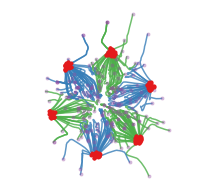
\includegraphics[width=.2\textwidth]{arxiv_figures/stdGauss_cycle2_6_linear_rect_0_steps.png} 
   \hspace{-2em} 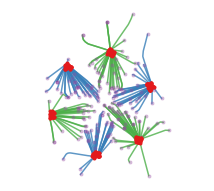
\includegraphics[width=.2\textwidth]{arxiv_figures/stdGauss_cycle2_6_linear_rect_1_steps.png} 
& 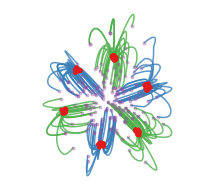
\includegraphics[width=.2\textwidth]{arxiv_figures/stdGauss_cycle2_6_vpsde_rect_0_steps.png} 
 \hspace{-2em}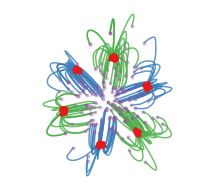
\includegraphics[width=.2\textwidth]{arxiv_figures/stdGauss_cycle2_6_vpsde_rect_1_steps.png} 
& 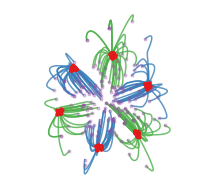
\includegraphics[width=.2\textwidth]{arxiv_figures/stdGauss_cycle2_6_sub_vpsde_rect_0_steps.png} 
    \hspace{-2em}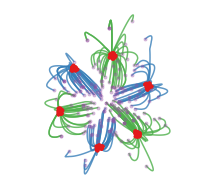
\includegraphics[width=.2\textwidth]{arxiv_figures/stdGauss_cycle2_6_sub_vpsde_rect_1_steps.png}  
\\
{\scriptsize \reflow{1}} \hfill
  {\scriptsize \reflow{2}} 
& {\scriptsize \reflow{1}} \hfill
 {\scriptsize \reflow{2}} 
& {\scriptsize \reflow{1}} \hfill
 {\scriptsize \reflow{2}} 
\end{tabular}
\caption{
Comparing rectified flow with VP ODE and sub-VP ODE when $\tg_0 = \normal(0,I)$ (purple dots) and $\tg_1$ is a low variance Gaussian mixture shown as the red dots. 
The linear rectified flow yields nearly straight trajectories with one step of reflow. But the trajectories of VP ODE and sub-VP ODE are curved and can not be straightened by reflowing. 
} 
\label{fig:gauss2dots}
\end{figure}


\newcommand{\trimlen}{1.5cm}
\begin{figure}[h]
    \centering
 \resizebox{\textwidth}{!}{    
\begin{tabular}{c|c|c|c|c}   
Time-Discretization & 
Rectified Flow & 
VP ODE & 
sub-VP ODE & 
VP ODE (const speed) \\
Steps $N$ & 
{\small $\alpha_t = t, \beta_t = 1-t$} & 
{\small $\alpha_t$ in \eqref{equ:vpode}, $\beta_t =\sqrt{1-\alpha_t^2}$} & 
{\small $\alpha_t$ in \eqref{equ:vpode}, $\beta_t = {1-\alpha_t^2}$}  & 
{\small $\alpha_t=t$, $\beta_t = \sqrt{1-\alpha_t^2}$} \\ \hline
 \small  $N=1$ & 
    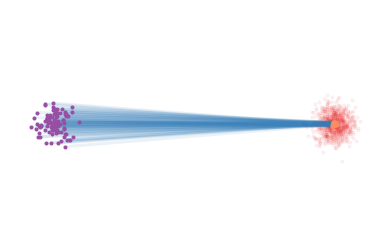
\includegraphics[width=.2\textwidth, trim={0cm 3cm 0 3cm},clip]{arxiv_figures/gg_linear_1steps.png} & 
    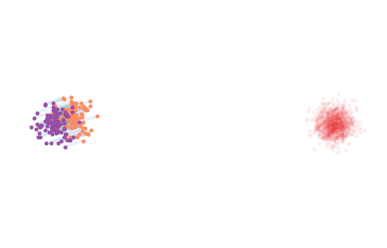
\includegraphics[width=.2\textwidth, trim={0cm 3cm 0 3cm},clip]{arxiv_figures/gg_vpsde_1steps.png} & 
    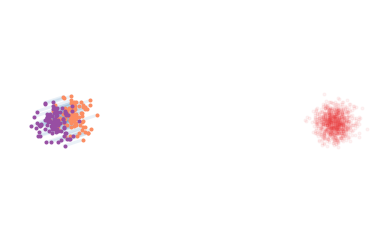
\includegraphics[width=.2\textwidth, trim={0cm 3cm 0 3cm},clip]{arxiv_figures/gg_sub_vpsde_1steps.png} & 
    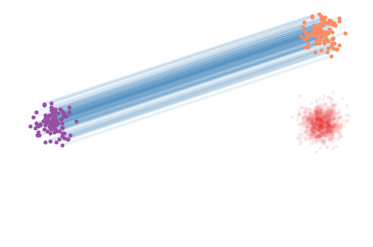
\includegraphics[width=.2\textwidth, trim={0cm 3cm 0 .4cm},clip]{arxiv_figures/gg_linear_prev_1steps.png}  \\  \hline  
    \small  $N=2$ &    
    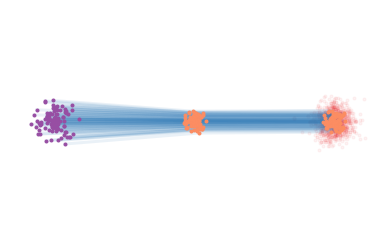
\includegraphics[width=.2\textwidth, trim={0cm 3cm 0 3cm},clip]{arxiv_figures/gg_linear_2steps.png} & 
        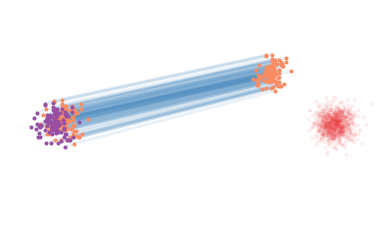
\includegraphics[width=.2\textwidth, trim={0cm 3cm 0 \trimlen},clip]{arxiv_figures/gg_vpsde_2steps.png} & 
        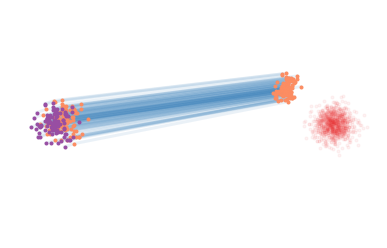
\includegraphics[width=.2\textwidth, trim={0cm 3cm 0 \trimlen},clip]{arxiv_figures/gg_sub_vpsde_2steps.png} & 
    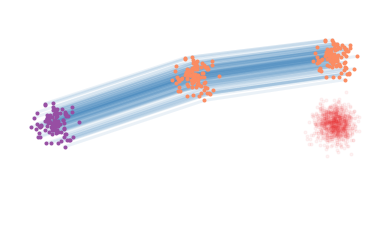
\includegraphics[width=.2\textwidth, trim={0cm 3cm 0 \trimlen},clip]{arxiv_figures/gg_linear_prev_2steps.png}  \\ \hline 
\small  $N=5$ &     
    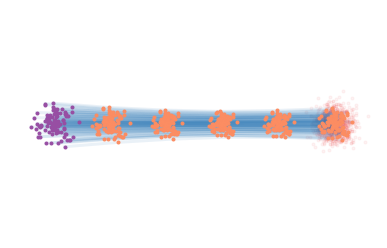
\includegraphics[width=.2\textwidth, trim={0cm 3cm 0 3cm},clip]{arxiv_figures/gg_linear_5steps.png} & 
    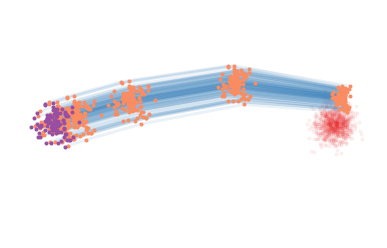
\includegraphics[width=.2\textwidth, trim={0cm 3cm 0 \trimlen},clip]{arxiv_figures/gg_vpsde_5steps.png} &     
    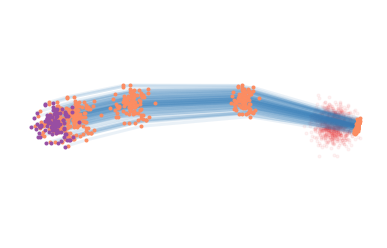
\includegraphics[width=.2\textwidth, trim={0cm 3cm 0 \trimlen},clip]{arxiv_figures/gg_sub_vpsde_5steps.png} &     
    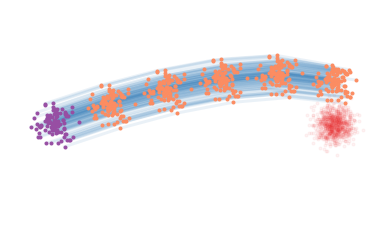
\includegraphics[width=.2\textwidth, trim={0cm 3cm 0 \trimlen},clip]{arxiv_figures/gg_linear_prev_5steps.png}  \\   \hline   
\small  $N=100$ &    
    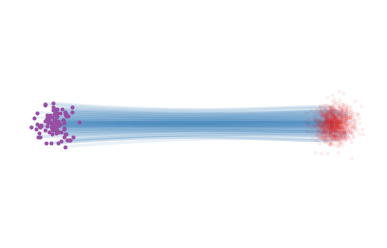
\includegraphics[width=.2\textwidth, trim={0cm 3cm 0 3cm},clip]{arxiv_figures/gg_linear_100steps.png} & 
    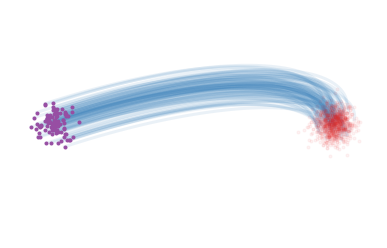
\includegraphics[width=.2\textwidth, trim={0cm 3cm 0 \trimlen},clip]{arxiv_figures/gg_vpsde_100steps.png} & 
    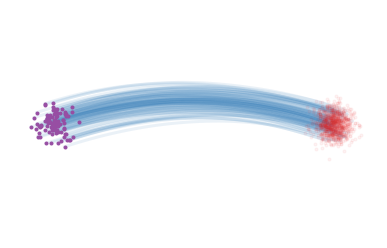
\includegraphics[width=.2\textwidth, trim={0cm 3cm 0 \trimlen},clip]{arxiv_figures/gg_sub_vpsde_100steps.png}  & 
    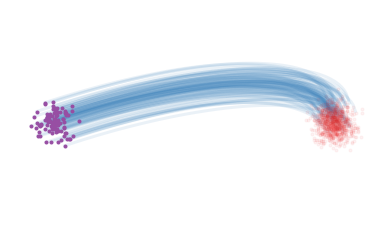
\includegraphics[width=.2\textwidth, trim={0cm 3cm 0 \trimlen},clip]{arxiv_figures/gg_linear_prev_100steps.png}     
\end{tabular}  
}
    \caption{Trajectories of different methods when varying the number of discretization steps $N$ (purple dots: $\tg_0$; red dots: $\tg_1$; orangle dots: intermediate steps; blue curves: flow trajectories).  
    The rectified flow travels in straight lines and progresses uniformly in time; 
    it generates the mean of $\tg_1$ when simulated with a single Euler step, and quickly covers the whole distribution $\tg_1$ with more steps (in this case $N=2$ is sufficient). %
    In comparison, 
    VP ODE and sub-VP ODE travel in curves with non-uniform speed: they tend to be slow in the beginning and speed up in the later phase (much of the update happens when $t{ \scriptstyle\gtrapprox}0.5$). The non-uniform speed can be avoided by setting $\alpha_t =t $ (see the last column). 
    }
    \label{fig:speedtoy}
\end{figure}


\paragraph{VP ODE and sub-VP ODE} 
The VP ODE and sub-VP ODE 
of \cite{song2020score}
 use the following shared $\alpha_t$: 
\bbb \label{equ:vpode}
\text{(sub-)VP ODE:}~~~~
\alpha_t = \exp\left (-\frac{1}{4} a(1-t)^2 %
- \frac{1}{2}b (1-t) 
\right );  && \text{default values: $a=19.9$, $b=0.1$,}
\eee  
where the default values of  $a,b$ are %
 chosen to match the continuous time limit of the shared training procedure of DDIM and DDPM. 
 The difference of VP ODE and sub-VP ODE is on the choice of $\beta_t$, given as follows:
\bbb \label{equ:vpodebeta} 
\text{VP ODE:~~~}\beta_t = \sqrt{1-\alpha_t^2},  &&
\text{sub-VP ODE:~~~}
\beta_t = {1-\alpha_t^2}. 
\eee  

As $\beta_0 \approx 1$ in both VP and sub-VP ODE, 
the $\tg_0$ in both cases are taken as  $\normal(0,I)$. %

The choices 
of $\alpha_t,\beta_t$ 
above  are the consequence of the 
SDE-based derivation in \cite{song2020score}. %
However, 
they are not well-motivated when we exam the path properties  of the induced  
ODEs:  %



\emph{$\bullet$~Non-straight paths:} 
Due to choices of $\beta_t$ in  \eqref{equ:vpodebeta}, the trajectories of VP ODE and sub-VP ODE are curved in general,  
and can not be straightened by the reflow procedure. 
We should choose 
 $\beta_t = 1-\alpha_t$ to induce straight paths. 


\begin{wrapfigure}{r}{0.4\textwidth}
  \vspace{-1\baselineskip}  
  \begin{center}
    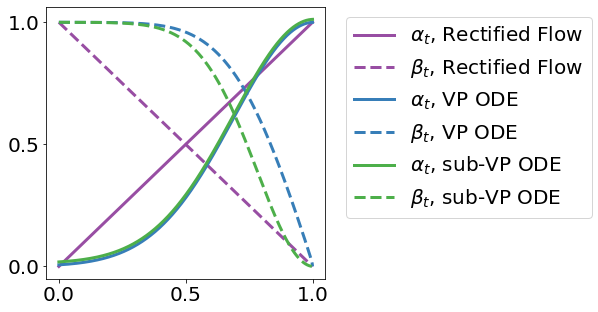
\includegraphics[width=0.4\textwidth]{arxiv_figures/alpha_beta.png}
  \end{center}
  \vspace{-.5\baselineskip}
  \caption{$t$ vs. $\alpha_t,\beta_t$ of different methods. 
  }
  \vspace{-.5\baselineskip}  
\end{wrapfigure}
\emph{$\bullet$~Non-uniform speed:} 
The exponential form of $\alpha_t$  in \eqref{equ:vpode} 
is a consequence of using  Ornstein–Uhlenbeck processes in the derivation of SDE models \cite{song2020score, ho2020denoising}.  
However, there is no clear advantage of using \eqref{equ:vpode} for  ODEs. 
As shown in Figure~\ref{fig:speedtoy},  
the $\alpha_t$ and $\beta_t$ of VP and sub-VP ODE 
change slowly in the early phase ($t{\scriptstyle \lessapprox} 0.5$).
As a result, 
the flow also moves slowly in beginning 
and hence most of the updates are concentrated in the later phase. 
Such non-uniform update speed, 
in addition to the non-straight paths,  
make VP ODE and sub-VP ODE perform sub-optimally 
when using large step sizes, even
for transport between simple spherical Gaussian distributions (see Figure~\ref{fig:speedtoy}).  
As we show in the last column of Figure~\ref{fig:speedtoy}, 
 changing the exponential $\alpha_t$ to the  linear function $\alpha_t = t$ in VP ODE 
 allows us to get a uniform update speed while 
 preserving the same continuous-time trajectories.






\paragraph{VE ODE} 
The VE ODE  of  \cite{song2020score} 
uses  
$\alpha_t = 1$ and 
$\beta_t = \sigma_{\min}\sqrt{r^{2(1-t)}-1}$   
where $\sigma_{\min} =0.01$ by default $r$ is set such that   $\sigma_{\max} \defeq r\sigma_{\min}$ is as large as the maximum Euclidean distance between all pairs of training data points from $\tg_1$  (Technique 1 of \cite{song2020improved}). 
Assume that %
$\sigma_{\max}^2$ 
is much larger than both $\sigma_{\min}^2$ and the variance of $X_1$,  
then  $X_0 = X_1 + \beta_0 \xi \approx \sigma_{\max}\xi $, and 
we can set the  initial distribution to be  $\tg_0\sim \normal(0,\sigma_{\max}^2 I)$, which has much larger variance than $\tg_1$. 
Hence, VE ODE can not be applied to (and not shown in) the toys in Figure~\ref{fig:gauss2dots} and Figure~\ref{fig:speedtoy}. 
As the case of (sub-)VP ODE, the restriction 
on $\xi$ is in fact unnecessary and requirement that $\sigma_{\max}$ is unnatural viewed from our framework. 
On the other hand, the trajectories of $X_t$ in VE ODE are indeed straight lines, 
because the direction of $\dot X_t = \dot \beta_t \xi$ is always the same as $\xi$. However, the choice of $\beta_t$ causes a  non-uniform speed issue similar to that of (sub-)VP ODE.  

Following \cite{song2020score, ho2020denoising}, a line of works have been proposed to improve the choices of $\alpha_t,\beta_t$, 
but remain to be constrained 
by the basic design space from the SDE-to-ODE derivation; see for example \cite{nichol2021improved, elucidating, zhang2022gddim}. 




To summarize, the simple nonlinear rectified flow framework in \eqref{equ:Lgvphi} 
both simplifies and extends the existing framework, and sheds a number of importance insights: %

$\bullet$~Learning ODEs can be considered directly and independently without resorting to diffusion/SDE methods; 

$\bullet$~The paths of the learned ODEs can be specified by any smooth interpolation curve $X_t$ of $X_0$ and $X_1$;  

$\bullet$~The initial distribution $\tg_0$ can be chosen arbitrarily, 
independent with the choice of 
the interpolation 
$X_t$.  

 $\bullet$~The canonical linear interpolation  $X_t = t X_1 + (1-t) X_0$ should be recommended as a default choice. 
 
On the other hand, non-linear choices of $X_t$ can be useful %
when we want to incorporate certain non-Euclidan geometry structure of the variable, 
or want to place certain constraints on the  trajectories of the ODEs.  
We leave this for future works. 
 













 




 
 


\section{Theoretical Analysis} 
\label{sec:theory}
We present the theoretical analysis for rectified flow. The results are summarized as follows. 


$\bullet$~[Section~\ref{sec:marginal}] %
All nonlinear rectified flows with any interpolation $X_t$ preserve the marginal laws.  

$\bullet$~[Section~\ref{sec:cost}] The rectified flow (with the canonical linear interpolation) reduces convex transport costs.  %

$\bullet$~[Section~\ref{sec:straight}] %
Reflow guarantees to straighten the (linear) rectified flows. 

$\bullet$~[Section~\ref{sec:stcouplings}] %
We clarify the relation between 
straight couplings and $c$-optimal couplings. 

$\bullet$~[Section~\ref{sec:diffusion}] We %
establish  PF-ODEs as instances of nonlinear rectified flows. 











 




 
 


\subsection{The Marginal Preserving Property}
\label{sec:marginal} 
The marginal preserving property that $\law(Z_t)=\law(X_t)$ for $\forall t$ is a general property of the nonlinear rectified flows in  \eqref{equ:Lgvphi},
regardless whether the interpolation $X_t$ is straight or not. 
\begin{mydef}
For a path-wise continuously differentiable random process  $\X = \{X_t\colon t\in[0,1]\}$, its expected velocity $v^\X$ is defined as 
$$v^\X(x, t) = 
\E[\dot X_t ~|~ X_t = x],~~~~~ \forall x\in \supp(X_t).
$$
For $x\not\in \supp(X_t)$, the conditional expectation is not defined and we set 
$v^\X$ arbitrarily, say $v^\X(x,t) = 0$. 
\end{mydef}

\begin{mydef}
We call that $\vv X$ is rectifiable if $v^\X$ is locally bounded and 
the solution of the integral equation below exists and  is unique: %
\bbb \label{equ:znonlinear} 
 Z_t = Z_0 + \int_0^t v^\X(Z_t, t) \dt,~~~~\forall t\in[0,1],~~~~ Z_0 = X_0.
\eee 
In this case, $\vv Z = \{Z_t\colon t\in[0,1]\}$ is called the rectified flow induced from $\vv X$. 
 \end{mydef}






\begin{thm}\label{thm:marginal}
Assume $\vv X$ is rectifiable and $\vv Z$ is its rectified flow. 
 Then  $\law(Z_t) =\law(X_t)$ for $\forall t\in[0,1]$. 
\end{thm}

\begin{proof} 
For any compactly supported continuously differentiable test function $h\colon \RR^d\to \RR$, we have 
\bbb  \label{equ:ehxt}
\ddt \E[h(X_t)]
 = \E[\dd h(X_t)\tt \dot X_t ] 
 = \E[\dd h(X_t)\tt v^\X(X_t,t)],  %
\eee  
where we used  $v^\X(X_t,t) = \E[\dot X_t |X_t]$.  
By definition, 
this %
is equivalent to that 
$\tg_t \defeq \law(X_t)$ solves 
in the sense of distributions the continuity equation with drift $v_t^\X \defeq v^\X(\cdot,t)$: 
\bbb \label{equ:contieq}
\dot \tg_t + \div (v_t^\X \tg_t) = 0.  
\eee 
To see the equivalence of \eqref{equ:ehxt} and \eqref{equ:contieq}, %
we can 
multiply \eqref{equ:contieq} with $h$ and integrate both sides:  
\bb 
0 = 
\int h(\dot \tg_t + \div (v_t^\X \tg_t)) 
= \int h \dot \tg_t - \dd h\tt v_t^\X \tg_t =  \ddt  \E[h(X_t) ]  - \E[\dd h(X_t)\tt v^\X(X_t,t)], 
\ee 
where we use integration by parts that $\int h\div (v^\X_t \tg_t)= - \int \dd h\tt (v^\X_t \tg_t)$. 

Because $Z_t$ is driven by the same velocity field $v^\X$, its  marginal law $\law(Z_t)$ solves the very same equation 
with the same initial condition ($Z_0=X_0$).  
Hence,  the equivalence of $\law(Z_t)$ and $\law(X_t)$ follows 
if the solution of \eqref{equ:contieq} is unique, 
which is equivalent to the uniqueness of the solution of $\d Z_t = \vofX(Z_t,t)$ following Corollary 1.3 of \citet{kurtz2011equivalence} (see also Theorem 4.1 of \citet{ambrosio2008existence}). 
\end{proof}











\subsection{Reducing Convex Transport Costs}
\label{sec:cost}
The fact that $(Z_0,Z_1)$ yields no larger convex transport costs than $(X_0,X_1)$ 
is a consequence of using the special linear interpolation $X_t = t X_1 + (1-t)X_0$ as the geodesic of Euclidean space. 

\begin{mydef}
A coupling $(X_0,X_1)$ is called rectifiable if its linear interpolation process $\vv X = \{tX_1+(1-t)X_0\colon t\in[0,1]\}$ is rectifiable. 
In this case, the 
$\vv Z=\{Z_t\colon t \in[0,1]\}$ in 
\eqref{equ:znonlinear} is called the 
rectified flow of coupling $(X_0,X_1)$, denoted as $\vv Z = \rectifyflow((X_0,X_1))$, 
and $(Z_0,Z_1)$ is called the rectified coupling of $(X_0,X_1)$, denoted as $(Z_0,Z_1) = \rectify((X_0,X_1)).$
\end{mydef}



\begin{thm} \label{thm:cost}
Assume $(X_0,X_1)$ is rectifiable and $(Z_0,Z_1) = \rectify((X_0,X_1))$. 
Then for any convex function $c\colon \RR^d\to \RR$, we have 
$$\E[c(Z_1 - Z_0)] \leq \E[c(X_1 - X_0)].$$ 
\end{thm} 
\begin{proof} 
The proof is based on elementary applications of Jensen's inequality. 
\bb
\E\left [c(Z_1 - Z_0)\right]
& = \E \left[ c\left(\int_0^1 \vofX(Z_t, t) \dt\right) \right ]  \ant{as $\d Z_t = \vofX(Z_t,t)\dt$}\\
&\leq \E \left[ \int_0^1 c \left (\vofX(Z_t, t)  \right) \dt \right ]  \ant{convexity of $c$, Jensen's inequality}\\
& = \E \left[ \int_0^1 c \left( \vofX(X_t, t)  \right) \dt \right ]  \ant{$X_t$ and $Z_t$ shares the same marginals}\\
& =  \E \left[ \int_0^1 c\left ( \E\left [(X_1-X_0)~|~X_t \right ] \right) \dt \right ] \ant{definition of $\vofX$}\\
& \leq  \E \left[ \int_0^1  \E\left [ c\left(X_1-X_0 \right) |~X_t \right ]   \dt \right ] \ant{convexity of $c$, Jensen's inequality}\\
& = \int_0^1\E\left [c\left(X_1 - X_0\right)\right] \dt  \ant{$\E[\E[(X_1-X_0) | X_t]] = \E[(X_1-X_0)]$}\\
& = \E\left [c\left (X_1 - X_0 \right) \right]. 
\ee 
\end{proof} 
 If $X_t$ is straight but with positive non-constant speed, that is, 
$X_t = \alpha_t X_1 + \beta_t X_0$ with $\beta_t = 1-\alpha_t$ and $\dot \alpha_t\geq0$, 
then we still have $\E[c(Z_1-Z_0)] \leq \E[c(X_1-X_0)]$ 
if $c$ is convex and $m$-homogeneous in that $c(a x) = \abs{a}^m c(x)$ 
for $\forall a\in \RR, x\in \RR^d$, with 
some constant $m\in(0, 1]$. 
 





\subsection{The Straightening Effect}
\label{sec:straight}


A coupling $(X_0,X_1)$ 
is said to be straight 
(or fully rectified)  if 
it is a fixed point of the $\rectify(\cdot)$ mapping.
It is desirable to obtain a straight coupling because its rectified flow is straight and 
hence can be simulated exactly with one step using numerical solvers. 
In this section, 
we first characterize the basic properties of straight couplings, showing that a coupling is straight iff its linear interpolation paths do not intersect with each other. Then, we prove that recursive rectification 
straightens the coupling and its related flow 
with a $\bigO{1/k}$ rate, where $k$ is the number of rectification steps. %


\begin{thm}\label{thm:straightness} 
Assume $(X_0,X_1)$ is rectifiable. Let $X_t =  tX_1 +(1-t)X_0$ and 
$\vv Z =\rectifyflow((X_0,X_1))$. 
Then $(X_0,X_1)$ is a straight coupling iff the following equivalent statements hold. %
\begin{enumerate} 
\item There exists a strictly convex function $c\colon \RR^d\to \RR$, such that $\E[c(Z_1-Z_0)] = \E[c(X_1-X_0)]$. 
\item $(X_0,X_1)$ is a fixed point of $\rectify(\cdot)$, that is, $(X_0,X_1) = (Z_0,Z_1)$. %
 
\item The rectified flow coincides with the linear interpolation process: $\vv X = \vv Z$. 

\item The paths of the linear interpolation $\vv X$ do not intersect: %
\bbb 
\hspace{-.05\textwidth}
V((X_0,X_1)):= 
\int_0^1 \e{\norm{X_1-X_0-\e{X_1-X_0~|~X_t}}^2} \dt = 0, 
\eee 
where %
 $V((X_0,X_1))=0$ 
 indicates 
 that $X_1-X_0=\E[X_1-X_0|X_t]$ almost surely when $t\sim \uniform([0,1])$, 
 meaning that the lines passing through each $X_t$ is unique, and hence no linear interpolation paths intersect. 
\end{enumerate}
\end{thm}
\begin{proof}

$3 \to 2\to 1$: Obvious. 



$1\to 4$: 
If $\E[c(Z_1-Z_0)] = \E[c(X_1-X_0)]$, the two applications of 
Jensen's inequality in the proof of Theorem~\ref{thm:cost}
are tight. Because $c$ is strictly convex,
the second Jensen's inequality in the proof implies that 
$X_1-X_0 = \E[X_1-X_0~|~X_t]$ almost surely w.r.t. $X$ and $t\sim \uniform([0,1]),$ which implies that $V(\vv X)=0.$

$4\to 3$:   
If $V(\vv X) =0$, we have $\int_0^s( X_1 -X_0) \dt = \int_0^s\E[X_1-X_0|X_t]\dt = \int_0^sv^X(X_t,t)\dt $ for $s\in(0,1]$.
Hence 
\bb 
X_t = X_0 +\int_0^t (X_1-X_0) \dt 
= X_0 + \int_0^t v^X(X_t, t) \dt. 
\ee 
Because $\vv Z$ satisfies the same equation 
\eqref{equ:znonlinear}, we have $\vv X=\vv Z$ by the uniqueness of the solution. 


\end{proof}




\paragraph{$\bigO{1/K}$ convergence rate}  
We now show that as we apply rectification recursively, 
the rectified flows become increasingly straight and the linear interpolation of the couplings becomes increasingly 
non-intersecting. 
\begin{thm} \label{thm:convergence} 
 Let $\vv Z^k$ the $k$-th rectified flow    
 of $(X_0,X_1)$, 
that is, $\vv Z^{k+1} = \rectifyflow((Z_0^k, Z_1^k))$ and $(Z_0^0,Z_1^0) = (X_0,X_1)$. 
Assume each $(Z_0^k,Z_1^k)$ is rectifiable for $k=0,\ldots, K$.  

Then %
\bb 
\sum_{k=0}^K 
S(\vv Z^{k+1}) + V( (Z^k_0, Z^k_1))
\leq  \e{\norm{X_1-X_0}^2}.
\ee 
 \end{thm}
 Hence, $\E[\norm{X_1-X_0}^2]<+\infty$,  we have 
 $\min_{k\leq K} (S(\vv Z^k) + V((Z_0^k,Z_1^k)) = \bigO{1/K}$. 
 
 
\begin{proof}
Taking  $c(x) = \norm{x}^2$ in 
the proof of Theorem 3.5, we can obtain that 
\bbb  \label{diff}
\e{\norm{X_1-X_0}} - \e{\norm{Z_1-Z_0}} = S(\vv Z) + V((X_0,X_1)).
\eee  
Applying it to each rectification step yields
$$
\E\left [\norm{Z^k_1-Z^k_0}^2\right ] - \E\left [\norm{Z^{k+1}_1-Z^{k+1}_0}^2\right ] = S(\vv Z^{k+1}) + V((Z_0^k,Z_1^k)). 
$$
A telescoping sum on $k=0,\ldots, K$ gives the result. 

\end{proof}


\subsection{Straight vs. Optimal Couplings} 
\label{sec:stcouplings}

A coupling $(X_0,X_1)$ is called $c$-optimal if it achieves the minimum of $\E[c(X_1-X_0)]$ among all couplings that share the same marginals.   
Understanding and computing the optimal couplings 
have been the main focus of optimal transport \cite[e.g.,][]{villani2009optimal,ambrosio2021lectures, figalli2021invitation, peyre2019computational}. 
Straight couplings is a different desirable property. %
In the following, 
we show that straightness is a necessary but not sufficient condition of being $c$-optimal for a strictly convex function $c$, except in the one dimensional case when the two concepts coincides. 
Hence, it is ``easier'' to find a straight coupling than a $c$-optimal couplings. 

\begin{thm}\label{thm:straightOpt}
If a rectifiable  coupling $(X_0,X_1)$ 
is $c$-optimal for some strictly convex cost function $c$, then $(X_0,X_1)$ is a straight coupling. 
\end{thm}
\begin{proof}
Let $(Z_0,Z_1) = \rectify((X_0,X_1))$. 
If $(X_0,X_1)$ is $c$-optimal, we must have $\E[c(Z_1-Z_0)] = \E[c(X_1-X_0)]$. 
This implies Statement 1 in Theorem \ref{thm:straightness} and hence that $(X_0,X_1)$ is straight. 
\end{proof}


\paragraph{1D Case}  
For any $\tg_0,\tg_1$ on $\RR$, there exists an unique coupling $(X_0^*,X_1^*)$
that is simultaneously optimal for all non-negative convex cost functions $c$. This coupling is uniquely characterized by a monotonic property: for every $(x_0,x_1)$ and $(x_0',x_1')$  in the support of $(X_0^*, X_1^*)$, 
if  $x_0< x_0'$, then $x_1 \leq x_1'$. 
Furthermore, if $\tg_0$ is absolutely continuously w.r.t. the Lebesgue measure, 
then $(X_0^*, X_1^*)$ must be deterministic in that there exists a mapping $T\colon \RR\to\RR$ such that $X_1^* = T(X_0^*)$. 
See \cite{santambrogio2015optimal}.   

In the following, we show that straight couplings on $\RR$ coincides with the deterministic monotonic coupling $(X_0^*, X_1^*)$ and hence is unique and simultaneously optimal for all convex $c$ when $\tg_0$ is absolutely continuous.
The idea is that, in $\RR$, a coupling is monotonic 
iff 
its linear interpolation paths do not intersect, a characteristic feature of straight couplings. 
\begin{lem}\label{thm:monostraightlemma}
A coupling on $\RR$ is  straight iff it is deterministic and monotonic. 
\end{lem} 
\begin{thm}\label{thm:1dstraight} 
For any $\tg_0,\tg_1$ on $\RR$, 
there exists either no straight coupling,
or a unique straight coupling. 
Further, if exists, the unique straight coupling is  deterministic and monotonic,  and jointly optimal w.r.t. all  convex cost functions $c\colon \RR^d\to [0,+\infty)$ 
for which the minimum value of $\e{c(X_1-X_0)}$ exists and is finite.  
\end{thm} 
\begin{proof}[Proof of Lemma~\ref{thm:monostraightlemma}] 
If $(X_0,X_1)$ on $\RR$ is straight, 
then it coincides with its rectified coupling $(Z_0,Z_1) = \rectify((X_0,X_1)).$ 
But because $(Z_0,Z_1)$ is induced from the rectified flow $\d Z_t = v^X(Z_t, t) \dt $, it is obviously deterministic. It is also monotonic due to the non-crossing property of flows.  Specifically, 
if $(Z_0,Z_1)$ is not monotonic, there exists $(z_0,z_1)$ and $(z_0',z_1')$ in the support of $(Z_0,Z_1)$ such that $z_0<z_0'$ and $z_1 > z_1'$. If this happens, there must exists $t_0\in(0,1)$, such that $z_{t_0} = z_{t_0}'$. But by the uniqueness of the solution, we have $z_t=z_t$ for $t\geq t_0$, which is conflicting with $z_1 > z_1'$. 

Assume $(X_0,X_1)$ is deterministic and monotonic. %
Due to the monotonicity, there exists no $x_0$ and $x_0'$ in the support of $\tg_0$, such that $x_0 \neq x_0'$ and $x_{t_0} = x_{t_0}'$ for some $t_0<1$.  This suggests that $X_1-X_0 = \E[X_1-X_0~|~X_t] = v^X(X_t,t)$ for $t\in(0,1)$, and hence  $\d  X_t = (X_1-X_0)\dt = v^X(X_t) \dt $, which is the ODE of the rectified flow. In addition, $X_t$ is obviously the unique solution of this ODE.  Hence $(X_0,X_1)$ is rectifiable and straight following Statement 3 of Theorem~\ref{thm:straightness}.  
\end{proof} 

\begin{proof}[Proof of Theorem~\ref{thm:1dstraight}]
This is the result of Lemma~\ref{thm:monostraightlemma} combined with the fact that the monotonic coupling is unique and jointly optimal for all convex $c$ for which the optimal coupling exists, following 
Lemma 2.8 and 
Theorem 2.9 of \cite{santambrogio2015optimal}. 
\end{proof}

\paragraph{Multi-dimensional cases} 
On the other hand, 
on $\RR^d$ with $d\geq 2$, 
the different cost functions $c$  do not share a common optimal coupling in general, 
and a straight coupling is not guaranteed to optimize 
a specific $c$; this is expected because the $\rectify(\cdot)$ procedure does not depend on a particular choice of $c$.
Hence, one must modify the $\rectify(\cdot)$ procedure 
to tailor it to a specific $c$ of interest. 


In a recent work 
\cite{khrulkov2022understanding}, 
it was  conjectured that the couplings $(Z_0,Z_1)$ induced from VP ODE (equivalently DDIM) yields an optimal coupling w.r.t. the quadratic loss, which was proved to be false in  \cite{lavenant2022flow, tanana2021comparison}. 
Here we show that 
even straight couplings 
are not guaranteed to be optimal, not to mention that VP ODE does not follow straight paths by design. 

We explore this in a separate work  \cite{rectifyOT} that is devoted to
modifying rectified flow to  find 
$c$-optimal couplings;
a result 
from \cite{rectifyOT} 
that can be easily stated 
is that 
the optimal coupling 
w.r.t. the quadratic cost $c(\cdot)=\norm{\cdot}^2$ 
can be achieved as the fixed point of $\rectify(\cdot)$ 
if $v$ is restricted to be a gradient field of form $v(x,t) = \dd f(x,t)$ 
when solving \eqref{equ:mainf}. Restricting $v$ to be a gradient field removes the rotational component of the velocity field $v^\X$ that causes sub-optimal transport cost.

 


